\documentclass[11pt]{article}
\usepackage[utf8]{inputenc}
\usepackage{graphicx}
\usepackage{caption}
\usepackage{subcaption}
\usepackage{amsmath}
\usepackage{float}


\title{
	{Computer Vision 2 - Assignment 1\\
	 Iterative Closest Point - ICP}
}
\author{
Selene Baez Santamaria (10985417) - Ildefonso Ferreira (10254757)}
\date{\today}

\begin{document}

\maketitle

\section{ICP}
In this assignment we create a function called \textit{ICP} which implements the Iterative Closest Point algorithm. This function takes as arguments a base point cloud and a target point cloud, and parameters like $k$ for the number of points to be sampled, $theshold$ for the precision desired, and $iter$ for the maximum number of iterations that should be run. It outputs the base point cloud, the transformed point cloud, and the rotation and transformation matrices.

\subsection{Implementation}
Our implementation follows the basic steps outlined by \texttt{Cai et al}. The steps are further explained in the following list:

\begin{enumerate}
	\item \textbf{Find closest points:} In this phase we find the corresponding points in the clouds. To do so we use the function provided by the assignment package \textit{dist2} to find the distance among two sets of points. For each point in the base cloud we match it with the point in the target cloud that returns the lowest distance. 
	
	Our first approach was to use brute force and compare all points in one cloud to the points in the second cloud. However, this lead to problems regarding memory capacity. Thus, we chose to sample the points to be matched to work within such limitations.
	
	A second approach led us to sample the first \textit{k} elements in each cloud and compare them. This leas to incomplete clouds which were not representative of the whole.
	
	Finally, we decided to go with uniform random sampling to get $k$ samples from each cloud, and match them together. This by itself brings new problems which shall be discussed in Section \ref{reflection}
	
	\item \textbf{Center point clouds:} Secondly, we find the geometric centers of each cloud and subtract the centroid from each point. 
	
	\item \textbf{Matrix Decomposition:} Next, we apply Singular Value Decomposition using Matlab's built in function \textit{svd}. The matrix to be decomposed is $A$, dimensions $3 x 3$, which is built as the dot product of the centered clouds: 
	
	\begin{center}
		$A = centered\_pcd\_base^T * centered\_pcd\_match$
	\end{center}
	
	The resulting matrices are the standard $U, S, V$ matrices.	
	
	\item \textbf{Find transformation matrices:} We proceed to calculate the Rotation and Translation matrices. 
	
	Since at every iteration we perform an update on the transformation of the target cloud, all of these updates must be combined to create the final matrices. For the rotation matrix this means each intermediate matrix should be multiplied with the accumulated matrix. For the translation matrix this means each intermediate matrix must be added to the accumulated matrix.
	
	\item \textbf{Transform matrix and evaluate:} Finally we calculate the average distances between the base and the transformed clouds. 
	
	We implemented two smart stopping conditions: the first stops if the distance is already within a certain threshold. The second condition limits the number of iterations to $iter$, since literature shows that there is a point after which the rate of significant improvement slows down and the improvement is insignificant.
\end{enumerate}

We tested our implementation with the given \textit{source.mat} and \textit{target.mat} files. The selected threshold is $ threshold = 0.00005 $, and the maximum number of iterations are $iter = 30$. In Figure \ref{fig:test} we present a visualization of the results obtained with these point clouds while Figure \ref{fig:test_performance} shows the performance on the algorithm per iteration.

\begin{figure}[H] \centering
	\begin{subfigure}{.5\textwidth} 
		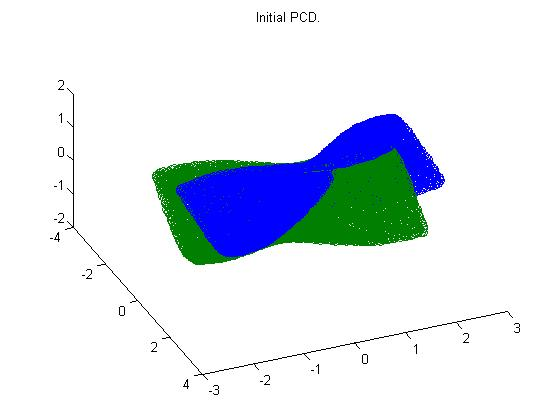
\includegraphics[width=.9\textwidth]{img/initial_test.jpg}
		\caption{Original source and target point clouds provided.}
	\end{subfigure}%
	\begin{subfigure}{.5\textwidth} 
		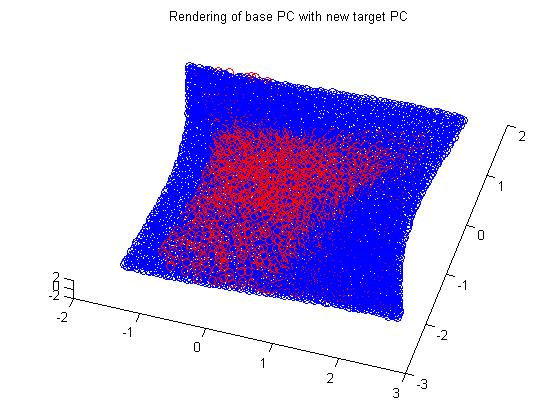
\includegraphics[width=.9\textwidth]{img/test_clouds.jpg}
		\caption{Alignment of source and target point clouds provided.}
		\label{fig:test}
	\end{subfigure}
	\caption{Testing the ICP function. Blue points correspond to source cloud and green points correspond to target cloud}
\end{figure}

\begin{figure}[H]
	\centering
	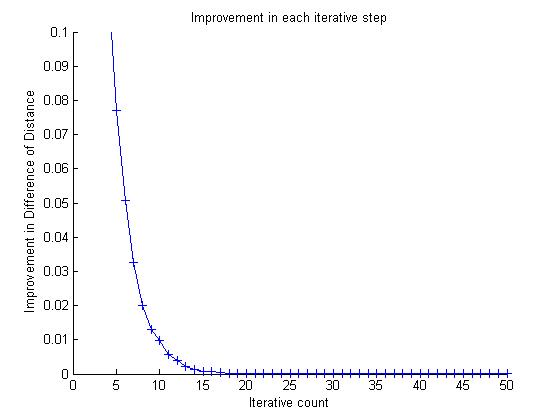
\includegraphics[width=.5\textwidth]{img/test_performance.jpg}
	\caption{Average distance between matched points per iteration for source and target test datasets.}
	\label{fig:test_performance}
\end{figure}


\section{Merging scenes}
We use our function on the dataset provided. The set consists of 100 frames, where each point cloud corresponds to the image of a person from different angles.

Before calling our function, we pre-process the frames and remove outliers points. Since the cloud contains noise regarding the background we ignore all points which third coordinate is larger than a threshold. After tuning we decided to set $ distance\_threshold = 1.5 $

Next, we created a function that merges two given frames. An example for merging Frame 1 and Frame 2 is in Figure \ref{fig:simple_consecutive}. 

\begin{figure}[H]
	\centering
	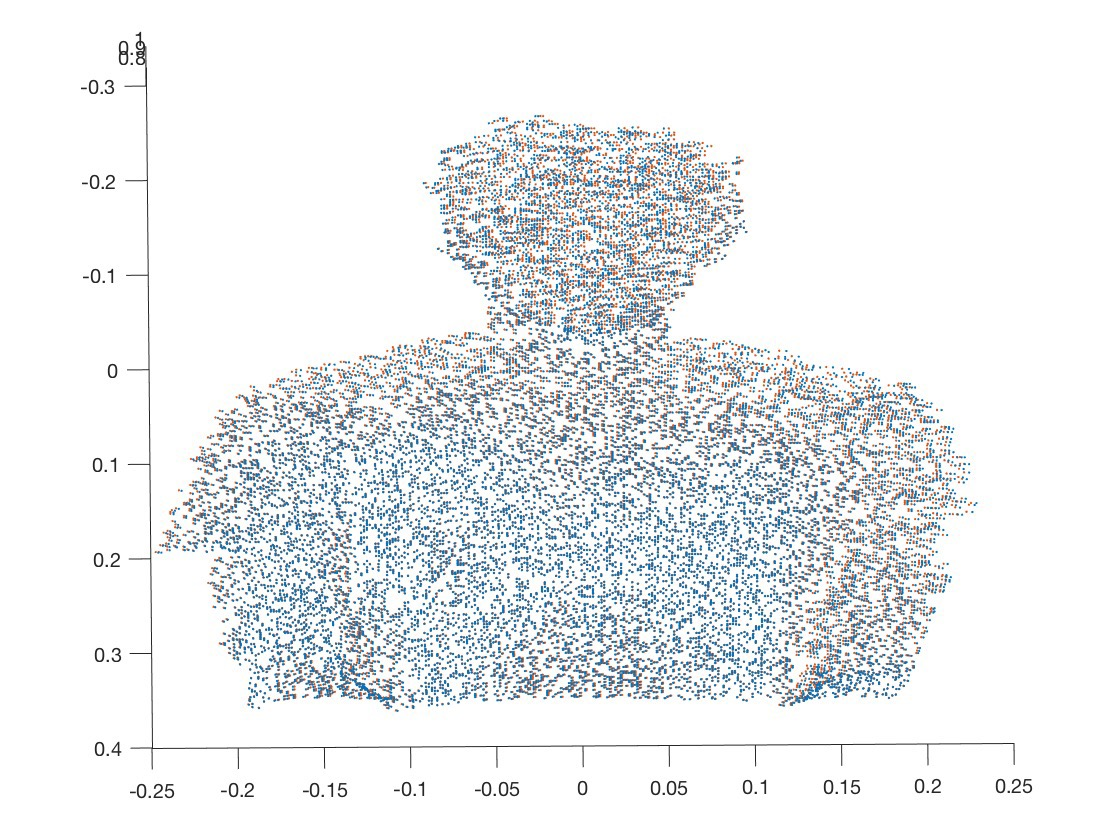
\includegraphics[width=.5\textwidth]{img/consecutive_matched.jpg}
	\caption{Average distance between matched points per iteration for source and target test datasets.}
	\label{fig:simple_consecutive}
\end{figure}

We perform two experiments to obtain estimate the camera poses: firstly we use consecutive frames and the second doing iterative merging. Due to computational complexity limitations, we relaxed the conditions and select these parameters: $ threshold = 0.001 $, and $iter = 10$.

\subsection{Consecutive frames}
Here we take the frames n a consecutive manner, skipping every $N$ frames. This means that the base for a targeted frame will always be the previous un-merged frame.

Results for $N = 10$ are shown in Figures \ref{fig:consecutive_10} and \ref{fig:consecutive_10_performance}. Similar results were obtained for $N = 2, 4$, with the only changes being a smoother performance graph and a more crowded visualization.

\begin{figure}[h] \centering
	\begin{subfigure}{.5\textwidth} 
		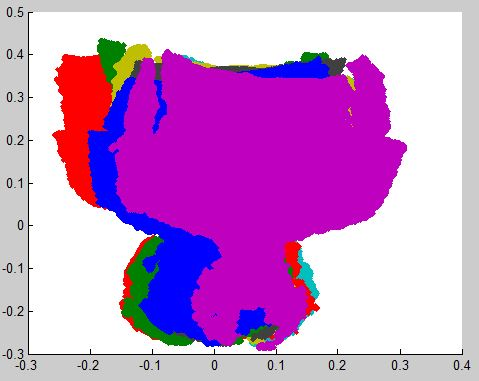
\includegraphics[width=.9\textwidth]{img/consecutive_10.jpg}
		\caption{Visualized transformed point clouds. Each point cloud is represented in a different color.}
		\label{fig:consecutive_10}
	\end{subfigure}%
	\begin{subfigure}{.5\textwidth} 
		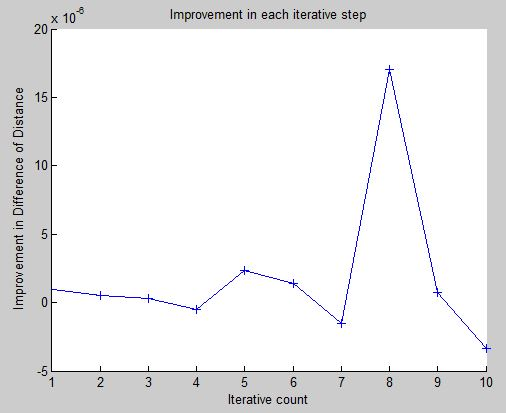
\includegraphics[width=.9\textwidth]{img/consecutive_10_performance.jpg}
		\caption{Performance graph showing average distance between matched points between pairs of consecutive frames.}
		\label{fig:consecutive_10_performance}
	\end{subfigure}
	\caption{Results for merging consecutive frames given $N = 10$.}
\end{figure}

We note that the camera parameters change for each consecutive pair of frames, which makes sense because the transformation between two frames can (and most likely does) vary. We also note that some frames do not align nicely, as shown by the shifted clouds  in the visualization. The performance graph supports this observation since the mean distance between consecutive frames increases suddenly for some pairs of frames. We suspect this is partly because of the inevitable drawbacks of ICP as well as our implementation detail, (e.g. the relaxation of the parameters). Further discussion is provided in Section \ref{reflection}.

\subsection{Iterative merging}
Again we take only frames in a consecutive manner skipping every $N$ frames. However, this time the base cloud for a targeted frame consisted of the merged clouds for all consecutive points. 

Results for $N = 10, 2$ are shown in Figure \ref{fig:iterative_2}, \ref{fig:iterative_2_performance} and Figure \ref{fig:iterative_10}, \ref{fig:iterative_10_performance} respectively. Runs for $N = 4$ are not included since they show the intermediate behavior between the previous two.

\begin{figure}[h] \centering
	\begin{subfigure}{.5\textwidth} 
		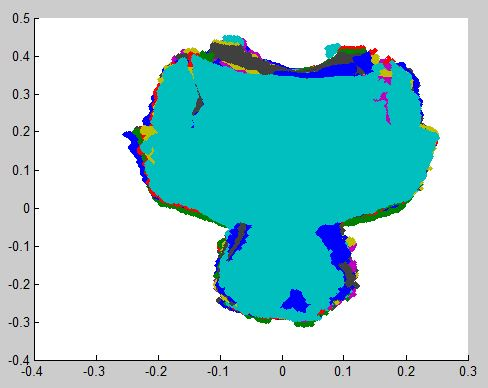
\includegraphics[width=.9\textwidth]{img/iterative_2.jpg}
		\caption{Visualized transformed point clouds. Each merge is represented in a different color.}
		\label{fig:iterative_2}
	\end{subfigure}%
	\begin{subfigure}{.5\textwidth} 
		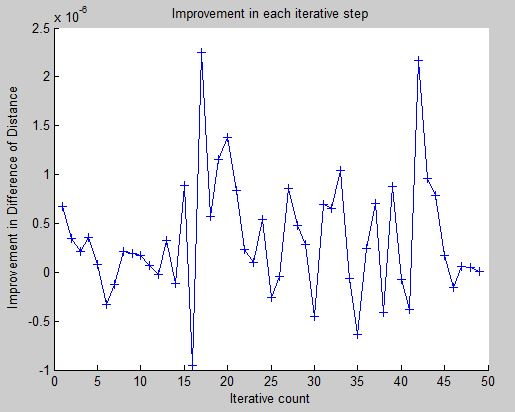
\includegraphics[width=.9\textwidth]{img/iterative_2_performance.jpg}
		\caption{Performance graph showing average distance between matched points between pairs of frames.}
		\label{fig:iterative_2_performance}
	\end{subfigure}
	\caption{Results for iterative merging of accumulated frames given $N = 2$.}
\end{figure}


\begin{figure}[h] \centering
	\begin{subfigure}{.5\textwidth} 
		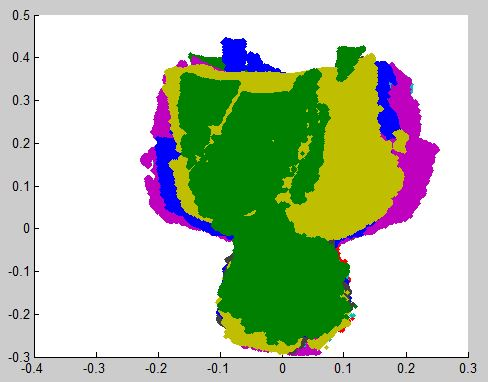
\includegraphics[width=.9\textwidth]{img/iterative_10.jpg}
		\caption{Visualized transformed point clouds. Each merge is represented in a different color.}
		\label{fig:iterative_10}
	\end{subfigure}%
	\begin{subfigure}{.5\textwidth} 
		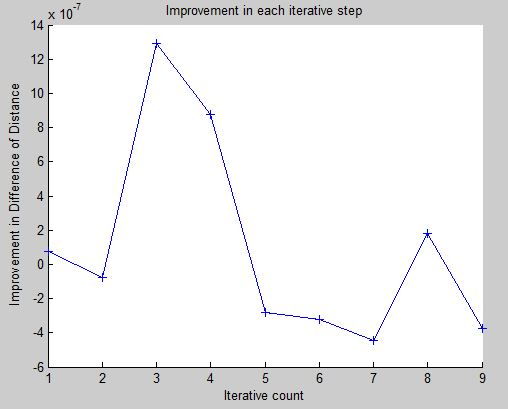
\includegraphics[width=.9\textwidth]{img/iterative_10_performance.jpg}
		\caption{Performance graph showing average distance between matched points between pairs of frames.}
		\label{fig:iterative_10_performance}
	\end{subfigure}
	\caption{Results for iterative merging of accumulated frames given $N = 10$.}
\end{figure}

We note that this time the camera parameters do not change as much during the experiment, but rather get refined as more frames are added. The explanation for this behavior is that by having an already merged point cloud as base, a new target base has more points available to be matched to. However, the performance graph shows that the error is higher for this experiment set up, which is at first glance counterintuitive. Our explanation for such behavior is that since this algorithm is trying to align one individual frame to an already accumulated model, the matching will be better thus making the transformation matrices will be more aligned to the general model; however, the trade is that such accumulated model is 'rougher' and loses detail as more frames are added. 

This explanation is supported by comparing the results from $N = 2$ with more frames than $N = 10$. As it is shown, the model with more frames is more rounded and does not contain much detail regarding the edge of the head and the shoulders. 

In conclusion, less frames lead to a more detailed model although chosen performance measure increases. The reason for the behavior of the performance measure is explained in the following section.

\section{Discussion}
\label{reflection}
Given the previous results we can reflect on our implementation and on the ICP algorithm in general.

\subsection{Reflection}
We noticed that the base cloud does not change over the iterations of the ICP, and so we thought that calculating and shifting the cloud once, in the first iteration of the algorithm, would suffice. On the other hand, since the target cloud does change, we calculate its centroid on every iteration and subtract it from every point. However, this approach led to errors in the transformation. After some reflection we realized our assumption was wrong. Since we performed the matching before the centering on every iteration, we were matching the centered base cloud with the un-centered target cloud.

Additionally we noticed that normalizing the rotation matrix did not have an effect on the end result or performance of the ICP function. Intuitively, we believed that normalizing would remove noise from the algorithm, however, this is not the case. 

\subsection{Drawbacks of ICP}
ICP heavily depends on the sampling process. Both the method and the size of the set are important. Given the memory complexity of the brute force comparison, we have to work within a certain limit of comparisons. It is a design choice to make a full comparison between a small sample set of selective comparisons between a large sample set. There is no guidelines on this, and literature provides methodology for the first type, called \textit{Selecting}, and the second type called \textit{Weighting}.

Additionally, the matching of the points is a highly non-convex problem which is subject to many local minima. Therefore, the position of the initial point clouds is crucial for the performance of the algorithm. If the initial orientation of the target is far from the base cloud, then the algorithm will get trapped in a local minimum.
 
 
\subsection{Improvements}
With regards to our implementation, we recognize that the sampling process could be improved. Random sampling does not ensure that the best most significant points will be taken into account while matching. A smarter approach is to select points according to their normals or other feature information, as suggested in the literature. However, given the time limitations we were not able to implement such mechanisms.

Additionally, we noted that the rotation matrices we obtained for the real dataset were not 100\% precise, since our main diagonal did not consist of $1$s but values close to it. A sample transformation matrix illustrating this is shown in Figure \ref{fig:matrix}. The reasoning for it could be computational precision, which could be improved in future implementations.

\begin{figure}[H]
	\centering
	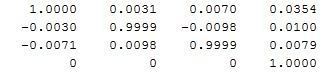
\includegraphics[width=.5\textwidth]{img/transformation_matrix.jpg}
	\caption{Sample of typical transformation matrix obtained with our ICP implementation}
	\label{fig:matrix}
\end{figure}

Furthermore, we could have improved the performance measure chosen. Currently we calculate the difference in the position of matched points and average them. However, some of the differences may be negative, which causes the average to shift in a non-representative way. We should have taken the absolute value of such differences to get the real distances between the points. This explains the behavior and interpretation of our performance graphs. Although it could be easily fixed, by the time we noticed the bug we could not perform the runs again due to time limitations.

In a more general scope, the ICP algorithm is very memory demanding, as it has been mentioned before. It makes sense that several improvements had been suggested to make smart selection of points and weighting of the matches. In it simplest, we can say that ICP is a very naive approach, guided by uninformed brute force. If treated as a search algorithm, ideas such as genetic algorithms or tabu search could find its parallel implementations in ICP.

\end{document}

